\begin{sepframe}{Functional code}
  {}
\end{sepframe}

\begin{frame}
  \frametitle{Functional code}
  \framesubtitle{Tips and tricks}

  \begin{itemize}[<+->]
    \item Make your objects \textbf{final},
    \item Make your properties \textbf{private} and \textbf{immutable},
    \item Make sure your functions are \textbf{total} and \textbf{pure}.
  \end{itemize}

  \note[item]{
    Some of you are getting to know me by now, and I couldn't make a
    presentation without discussing about functional code and how to
    improve your code with simple and basic tips like...
  }

  \note[item]{
    Since the last presentation we did and from the feedback that I had from
    colleagues, I noticed that the notion of final class is sometimes
    misunderstood. I'm going to show with an example why it is important to
    make sure that we can't extend classes.
  }

  \note[item]{
    Immutability is the trending word in I.T. since a couple of years now,
    and especially these last years. Its origin comes from
    the code and if we dig deeper, we will discover that it has roots in
    Lambda Calculus by Alonzo Church in 1930.
    Needless to say that making variables and objects immutable increase the
    ease of debugging and it is prone to the use of good design patterns.
  }

  \note[item]{
    Total functions are basically the gist of all of this including the
    reason why we have complexity and monads. I'm going to formalize the
    definition of them with a definition and some examples.
    I will also show what partial and pure functions are.
  }

\end{frame}

\begin{frame}
  \frametitle{Functional code}
  \framesubtitle{Final classes}

  \lstinputlisting[caption={Class is not final}]{src/session/functional/resources/immutability1-a.php}
  \pause
  \lstinputlisting[caption={When extending a class which is not final...}]{src/session/functional/resources/immutability1-b.php}
  \note[item]{
    When extending a class, it's easy to change the original behavior of a
    class. Sometimes, it's even possible to alter and completely change an
    original behavior. I guess this is a wrong idea, don't you think?
  }
\end{frame}

\begin{frame}
  \frametitle{Functional code}
  \framesubtitle{Final classes}

  \lstinputlisting[caption={Class is not final}]{src/session/functional/resources/immutability2-a.php}
  \pause
  \lstinputlisting[caption={When extending a class which is not final...}]{src/session/functional/resources/immutability2-b.php}

  \note[item]{
    Another example here, maybe a bit better.
  }
  \note[item]{
    When a class is not final, developers may be prone to extend them and
    introduce unwanted behaviors while keeping semantically the same thing.
  }
\end{frame}

\begin{frame}
  \frametitle{Functional code}
  \framesubtitle{Public and private properties}

  \lstinputlisting[caption={Public properties}]{src/session/functional/resources/properties1-a.php}
  \pause
  \lstinputlisting[caption={Private properties}]{src/session/functional/resources/properties1-b.php}

  \note[item]{
    A quick reminder here, I hope you're not learning something new on this
    slide!
  }

\end{frame}

\begin{frame}
  \frametitle{Functional code}
  \framesubtitle{Partial and total functions}

  A total function is a function which is defined for all inputs.

  \pause

  \begin{definition}[Total function]
    \begin{align*}
       & f: A \mapsto B                               \\
       & \forall a \in A \implies \exists\ f(a) \in B
    \end{align*}
  \end{definition}

  \note[item]{
    Here's a formal definition of a total function because sometimes a
    smaller and formal definition worth ten thousands words.
  }

  \note[item]{
    Let f a function which takes an input of type A and return a type B.
  }
  \note[item]{
    For all a in type A implies that it exist the image of a through f in
    type B.
  }
\end{frame}

\begin{frame}
  \frametitle{Functional code}
  \framesubtitle{Partial and total functions}

  A partial function is a function which is not defined for all inputs.

  \pause

  \begin{definition}[Partial function]
    \begin{align*}
       & f: A \rightharpoonup B                           \\
       & \exists x \in A \implies \not\exists\ f(x) \in B
    \end{align*}
  \end{definition}

  \note[item]{
    And now, a formal definition of a partial function. This was a bit
    more complex to find out and it might not be the best definition.
    But hey, I'm just a developer!
  }
  \note[item]{
    Let f a function which takes some input of type A and return a type B.
    The word "some" is very important here, you can see that the arrow is
    also a bit different.
  }
  \note[item]{
    It exists x in type A implying that it does not exists an image of x
    through f in type B.
  }
\end{frame}

\begin{frame}
  \frametitle{Functional code}
  \framesubtitle{Partial and total functions}

  \begin{definition}[Total function]
    \begin{align*}
       & f: A \mapsto B                              \\
       & \forall a \in A \implies \exists f(a) \in B
    \end{align*}
  \end{definition}

  \begin{definition}[Partial function]
    \begin{align*}
       & f: A \mapsto B                                  \\
       & \exists x \in A \implies \not\exists f(x) \in B
    \end{align*}
  \end{definition}

  \note[item]{
    Just for the beauty of the definitions, here they are, both of them.
  }
\end{frame}

\begin{frame}
  \frametitle{Functional code}
  \framesubtitle{Partial and total functions}

  \begin{itemize}
    \item Total: \lstinline[language=PHP]!function add (int $a, int $b): int!\pause
    \item Partial: \lstinline[language=PHP]!function divide(int $a, int $b): float!\pause
    \item Not pure: \lstinline[language=PHP]!time()!\pause
    \item Pure: \lstinline[language=PHP]!function add (int $a, int $b): int!
  \end{itemize}

  \note[item]{
    A very basic example of total and partial function now to make sure
    that the definition is well understood.
  }
  \note[item]{
    Tips: when making functions, methods, try to make total functions
    to reduce complexity later on.
    Total functions are definitely less trouble makers than partials.
  }
\end{frame}

\begin{frame}
  \Huge
  \begin{center}
    What\pause\ the\pause\ link\pause\ ????
  \end{center}

  \note[item]{
    Some of you might say... but what is this guy saying? Why is he telling
    us all these theoratical stuff that I vaguely remember from school ?!
  }
  \note[item]{
    Don't worry, everything will come at once, everything is actually linked
    together.
  }
  \note[item]{
    Please, let's keep all of that in mind an move on to more concrete
    examples.
  }
\end{frame}

\begin{frame}
  \frametitle{Functional code}
  \framesubtitle{Handling errors}

  \lstinputlisting[caption={A Doctrine repository definition}]{src/session/functional/resources/doctrine-repository1-a.php}
  \pause
  \lstinputlisting[caption={A Doctrine repository in use}]{src/session/functional/resources/doctrine-repository1-b.php}

  \note[item]{
    If you use Doctrine properly, this is the kind of stuff that you have
    all over your code.
    I don't know what you think, but this is usually where issues are
    coming. Why ?
    Simply because of the use of the null value. If the method find would
    not return null, then this check is definitely useless.
  }
  \note[item]{
    If we want to alter that behavior, then we need to rewrite some parts
    from Doctrine, which we really want to avoid for now.
  }
  \note[item]{
    Let's use another example not involving Doctrine.
  }
\end{frame}

\begin{frame}
  \frametitle{Functional code}
  \framesubtitle{Tips and tricks}

  \lstinputlisting[caption={Return null}]{src/session/functional/resources/square-root1-a.php}
  \pause
  \lstinputlisting[caption={Throw exception}]{src/session/functional/resources/square-root1-b.php}
  \pause
  \lstinputlisting[caption={Return sentinel}]{src/session/functional/resources/square-root1-c.php}

  \note[item]{
    This idea here is to create a safeSquareRoot function which would return
    the square root of any numeric value, and we have to deal with negative
    numbers. And how should we deal the negative values? What are the
    options?
  }
  \note[item]{
    The first option we have is to return the controversial null value when
    the input value is a negative number.
  }
  \note[item]{
    The second option is to throw an exception and potentially stop the
    program.
  }
  \note[item]{
    The third option is to return a sentinel value.
  }
\end{frame}

\begin{frame}
  \frametitle{Functional code}
  \framesubtitle{Tips and tricks}

  \begin{itemize}
    \item Return null?\pause
          \\\textcolor{ecgrey!50}{Mixing types implies more code for the end
            user, prevent composition.}
    \item Throw exceptions?\pause
          \\\textcolor{ecgrey!50}{Great power means great responsibility, has
            the power to stop the program.}
    \item Return sentinel?\pause
          \\\textcolor{ecgrey!50}{Prone to incertitude when it returns 0.}
  \end{itemize}

  \note[item]{
    Return null ... explain and give an example with Doctrine.
  }
  \note[item]{
    Exceptions are great, but needs to be correctly documented and handled.
  }
  \note[item]{
    Sentinels, avoid that, it's an old thing and extremelly prone to
    incertitude.
  }
\end{frame}

\begin{frame}
  \frametitle{Functional code}
  \framesubtitle{Return null?}

  \begin{itemize}[<+->]
    \item Universal error value that doesn't carry any relevant information
          in case of issues.
    \item Widespread, implemented in most languages
    \item Considered as a code smell and a "the billion-dollar mistake"
    \item Prevent composition pattern
  \end{itemize}

  \note[item]{
    Java, C,... implements nullable objects BY DEFAULT, controversial.
  }
\end{frame}

\begin{frame}
  \frametitle{Functional code}
  \framesubtitle{Throw exceptions?}

  \begin{itemize}[<+->]
    \item Indicate something unforeseen by the developer
    \item Expensive, destructive
    \item Definitely prevent composition pattern
  \end{itemize}

  \note[item]{
    Should be carefully used.
  }
\end{frame}

\begin{frame}
  \frametitle{Functional code}
  \framesubtitle{Return sentinel?}

  \begin{itemize}[<+->]
    \item Potentially prevent composition pattern
    \item Must be carefully done, each type has its own unit type
          \begin{itemize}[<+->]
            \item \lstinline[language=PHP]!function divide(int $a, int $b): float|string!
            \item \lstinline[language=PHP]!function divide(int $a, int $b): float|array!
            \item \lstinline[language=PHP]!function divide(int $a, int $b): float|null!
            \item \lstinline[language=PHP]!function divide(int $a, int $b): float|int!
          \end{itemize}
    \item In PHP, this is sadly happening
  \end{itemize}

  \note[item]{
    Ask the audience in which PHP function this happens ? (strpos)
  }
\end{frame}

\begin{frame}
  \frametitle{Functional code}
  \framesubtitle{What is our best option?}

  \begin{itemize}[<+->]
    \item Not using PHP ?
    \item Avoid using strict types ?
    \item Wrap the incertitude in a well-know object?
  \end{itemize}

  \note[item]{
    Take a break, let's make a summary of what we've seen (TODO)
  }

  \note[item]{
    AFAIK, there are no other options available. So, what is the best option
    here?
  }

  \note[item]{
    Well it depends.
    IMHO, there is no better option, but rather the least worst.
    In a way, all these options are breaking composition pattern so, they
    are almost useless. What does it means?
  }
  \note[item]{
    It means that you cannot stack functions calls one after the other.
    Composition pattern will prevent you to break the logic flow and
    checking the return value of the previous function before using it as
    input of the next one.
  }

  \note[item]{
    Start to slowly introduce the concept of monads using Schrodinger's cat.
  }
\end{frame}

\begin{frame}
  \begin{figure}
    \begin{overprint}
      \onslide<1>
      \begin{center}
        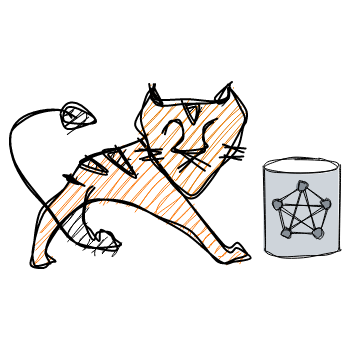
\includegraphics[width=10em]{src/session/functional/resources/cat.png}
      \end{center}
      \onslide<2->
      \begin{center}
        
\includegraphics[width=15em]{src/session/functional/resources/box.png}
      \end{center}
    \end{overprint}
  \end{figure}


  \note[item]{
    Let's make a mind experience now.
  }
  \note[item]{
    Do you know this famous cat? Yes, this is the Tomcat logo.
  }
  \note[item]{
    Next to the cat, there is a barrel of toxic waste. The cat could die if
    it were to play with the barrel and breathe in the toxic gases.
  }
  \note[item]{
    Now, let's put them in a sealed box.
  }
  \note[item]{
    After a couple of minutes, are you able to tell if the cat is alive or
    not?
  }
  \note[item]{
    The only way to tell if the cat is alive is to open the box, right?
    But maybe opening the box will cause the cat to die?
  }
  \note[item]{
    At this point, there is no way to tell if the cat is alive or not.
    The cat is dead and alive at the same time. This is the Schrodinger's
    cat.
  }
  \note[item]{
    What we're going to see next is basically the same thing.
  }
  \note[item]{
    How about the idea of abstracting the incertitude by creating an object
    that would wrap a value in a well-know object?
  }
  \note[item]{
    An object that can be \textbf{maybe} null or \textbf{maybe} the expected
    value... just like the Schrodinger's cat?
  }
  \note[item]{
    Let's make together this first object in PHP. This is where there will
    be a bit of code. Please stay focused.
  }
\end{frame}

\begin{frame}
  \lstinputlisting[caption={Maybe class directions}]{src/session/functional/resources/maybe-draft1-a.php}
\end{frame}

\begin{frame}
  \lstinputlisting[caption={Maybe class implementation and usage}]{src/session/functional/resources/maybe-draft1-b.php}
\end{frame}

\begin{frame}
  \lstinputlisting[caption={Maybe class with our snippet}]{src/session/functional/resources/maybe-draft1-c.php}
\end{frame}

\begin{frame}
  \lstinputlisting[caption={Maybe class with our snippet and callbacks}]{src/session/functional/resources/maybe-draft1-d.php}
  \note[item]{
    All of this is cool, but problem is still there.
  }
  \note[item]{
    Do you see it?
  }
  \note[item]{
    We are still writing partial functions and mixing types, we are back to
    square one.
  }
\end{frame}

\begin{frame}
  \lstinputlisting[caption={Draft Maybe class}]{src/session/functional/resources/maybe-draft1-e.php}

  \note[item]{
    We could fix this issue by just updating the "then" method as such...
  }
  \note[item]{
    In the previous version, we were wrapping the result of the method call
    in a new object, let's get rid of that and update our callbacks
    accordingly.
  }
\end{frame}

\begin{frame}
  \lstinputlisting[caption={Draft Maybe class}]{src/session/functional/resources/maybe-draft1-f.php}

  \note[item]{
    It's a bit more verbose for sure, but now all the callbacks are total
    functions!
  }
  \note[item]{
    As you can see, this is already nice, our snippet is a bit easier to
    read and to modify.
  }
\end{frame}

\begin{frame}
  \frametitle{Functional code}
  \framesubtitle{The Maybe class}

  \begin{itemize}[<+->]
    \item Is actually the ``Maybe'' monad,
    \item Focus on the happy scenario,
    \item Return \texttt{null} when something goes wrong,
    \item Unable to know the reason when something is wrong,
    \item Back to square 1.
  \end{itemize}

  \note[item]{
    Let's summarize a bit what we've seen here.
  }
  \note[item]{
    While using the maybe monad could be useful is some cases it might not
    be the best choice if you need to know why something has failed.
  }
\end{frame}

\begin{frame}
  \frametitle{Functional code}
  \framesubtitle{The Maybe class}

  Maybe we could customize the return value in case of something wrong happen?\\
  \vfill
  \pause
  While still being able to decide what to do when an error happen?
  \vfill
  \pause
  \begin{flushright}
    Let's hack !
  \end{flushright}
\end{frame}

\begin{frame}
  \lstinputlisting[caption={Either class direction}]{src/session/functional/resources/either-draft1-a.php}

  \note[item]{
    Let's update the maybe class and add the necessary changes.
  }
\end{frame}

\begin{frame}
  \lstinputlisting[caption={Either class usage}]{src/session/functional/resources/either-draft1-f.php}

  \note[item]{
    You may notice that the callbacks are total, nothing has changed except
    that we replaced the return types and added a "left" case when something
    wrong happen.
  }
  \note[item]{
    There is also a difference during the last method call at the end,
    the developer needs to submit a callback that will eventually deal with
    the potential exception.
  }
  \note[item]{
    If there is no exception, then the Either class will return the expected
    value, if not, it will execute the callback and pass the exception to it
    It's up the developer to do whatever he wants with the exception.
  }
\end{frame}

{
\setbeamercolor{background canvas}{bg=IcebergSky}
\begin{frame}[plain]
  \centering
  \vskip 0pt plus 1filll
  \Huge So these are monads !
  \vskip 0pt plus 1filll
  \makebox[\linewidth]{
\includegraphics[width=\paperwidth]{src/session/functional/resources/iceberg-top.png}}

  \note[item]{
    We are at the end of the presentation finally !
  }
  \note[item]{
    As you can see, I just introduced monads at the end of the slides
    because I think it is important to know a bit of context and history on
    where they come from in order to know how and where to use them.
  }
  \note[item]{
    What you see down there is a top of an iceberg, this is exactly what we
    did today. We just scratched the surface of this world. We discovered
    the two first monads Maybe and Either.
  }
  \note[item]{
    There's a lot to learn and discover, but it is not the intention of this
    presentation today. The idea here was to open some doors and introduce
    the concept, nothing else, nothing more.
  }
\end{frame}
}

{
\setbeamercolor{background canvas}{bg=IcebergDeepBlue}
\begin{frame}[plain]
  \makebox[\linewidth]{
\includegraphics[width=\paperwidth]{src/session/functional/resources/iceberg-bottom.png}}
  \centering
  \vskip 0pt plus 1filll
  \Large
  \begin{itquote}
    Technically, a monad is a monoid in the monoidal category of
    endofunctors equipped with functor composition as its product.
  \end{itquote}
  \vskip 0pt plus 1filll

  \note[item]{
    This is what you might encounter when going further with monads.
  }
  \note[item]{
    The theory behind monads are from the Category theory which is
    completely out of this World.
  }
\end{frame}
}

\begin{frame}
  \centering
  \Huge Should I use monads ?

  \note[item]{
    Depends on the language you're using, you might be already using them.
    In Java, you can use them through the Optional class, in Javascript with
    Promises, in PHP with... Argh !
    There is actually no ``official'' monad package and PHP developers are
    not used to program this way. However, there is a very good userland
    implementation: Lamphpda from Marco Perone.
  }
\end{frame}

\begin{frame}
  \frametitle{Functional code}
  \framesubtitle{State of PHP and monads}

  \begin{itemize}[<+->]
    \item No core implementation
    \item Only ``userland'' implementations
    \item Prone to static analysis
    \item Implementations:
          \begin{itemize}[<+->]
            \item \href{https://github.com/marcosh/lamphpda}{github.com/marcosh/lamphpda}
            \item \href{https://github.com/loophp/repository-monadic-helper/}{github.com/loophp/repository-monadic-helper/}
          \end{itemize}
  \end{itemize}
\end{frame}

\begin{frame}
  \frametitle{Functional code}
  \framesubtitle{Monads summary}

  \begin{itemize}
    \item Introduced in 1988 by Eugenio Moggi
    \item Maybe: Deal with a value and null
    \item Either: Deal with a value and another value
          Maybe is to some extent a specialization of Either.
    \item ...Reader, Writer, IO, List,... There are many other monads these
          two are just the tip of the iceberg.
    \item Monads may have different names in languages (Optional, Result, Promise, etc etc)
    \item Monads are the design pattern of functional languages
    \item Underlying theory can be very complex
    \item We don't need to understand them to use them !
  \end{itemize}
\end{frame}

\begin{frame}
  \centering
  \Huge Should I use monads ?
\end{frame}

\begin{frame}
  \frametitle{Functional code}
  \framesubtitle{Monads benefits}

  \begin{itemize}
    \item Monads can abstract most of your function binding, turning a lot of
          noise into magic.
    \item It modularizes logical unit of computation and facilitate refactoring
    \item Reduce complexity of the code, abstracting the logic into one well
          known object that does only thing.
    \item Either: Deal with a value and another value
    \item For educational purposes ? Demystifing monads can help understand
          the benefits and perks of functional programming, and make you a better
          developer.
  \end{itemize}
\end{frame}

\begin{frame}
  \centering
  \Huge Thank you all for listening!
\end{frame}
